%!TEX root = ../main.tex
\chapter{Validation: Additional Plots}
\label{appendix:SimulationVal}

\begin{figure}[htbp!]
  \centering
  \begin{subfigure}[t]{0.49\textwidth}
    \includegraphics[width=1.\linewidth]{../Thesis_Plots/Timing/Muons/Plots/BeamProfileX.pdf}
    \caption{Beam profile X.} \label{fig:mu150GeVX}
  \end{subfigure}
  \hfill
  \begin{subfigure}[t]{0.49\textwidth}
    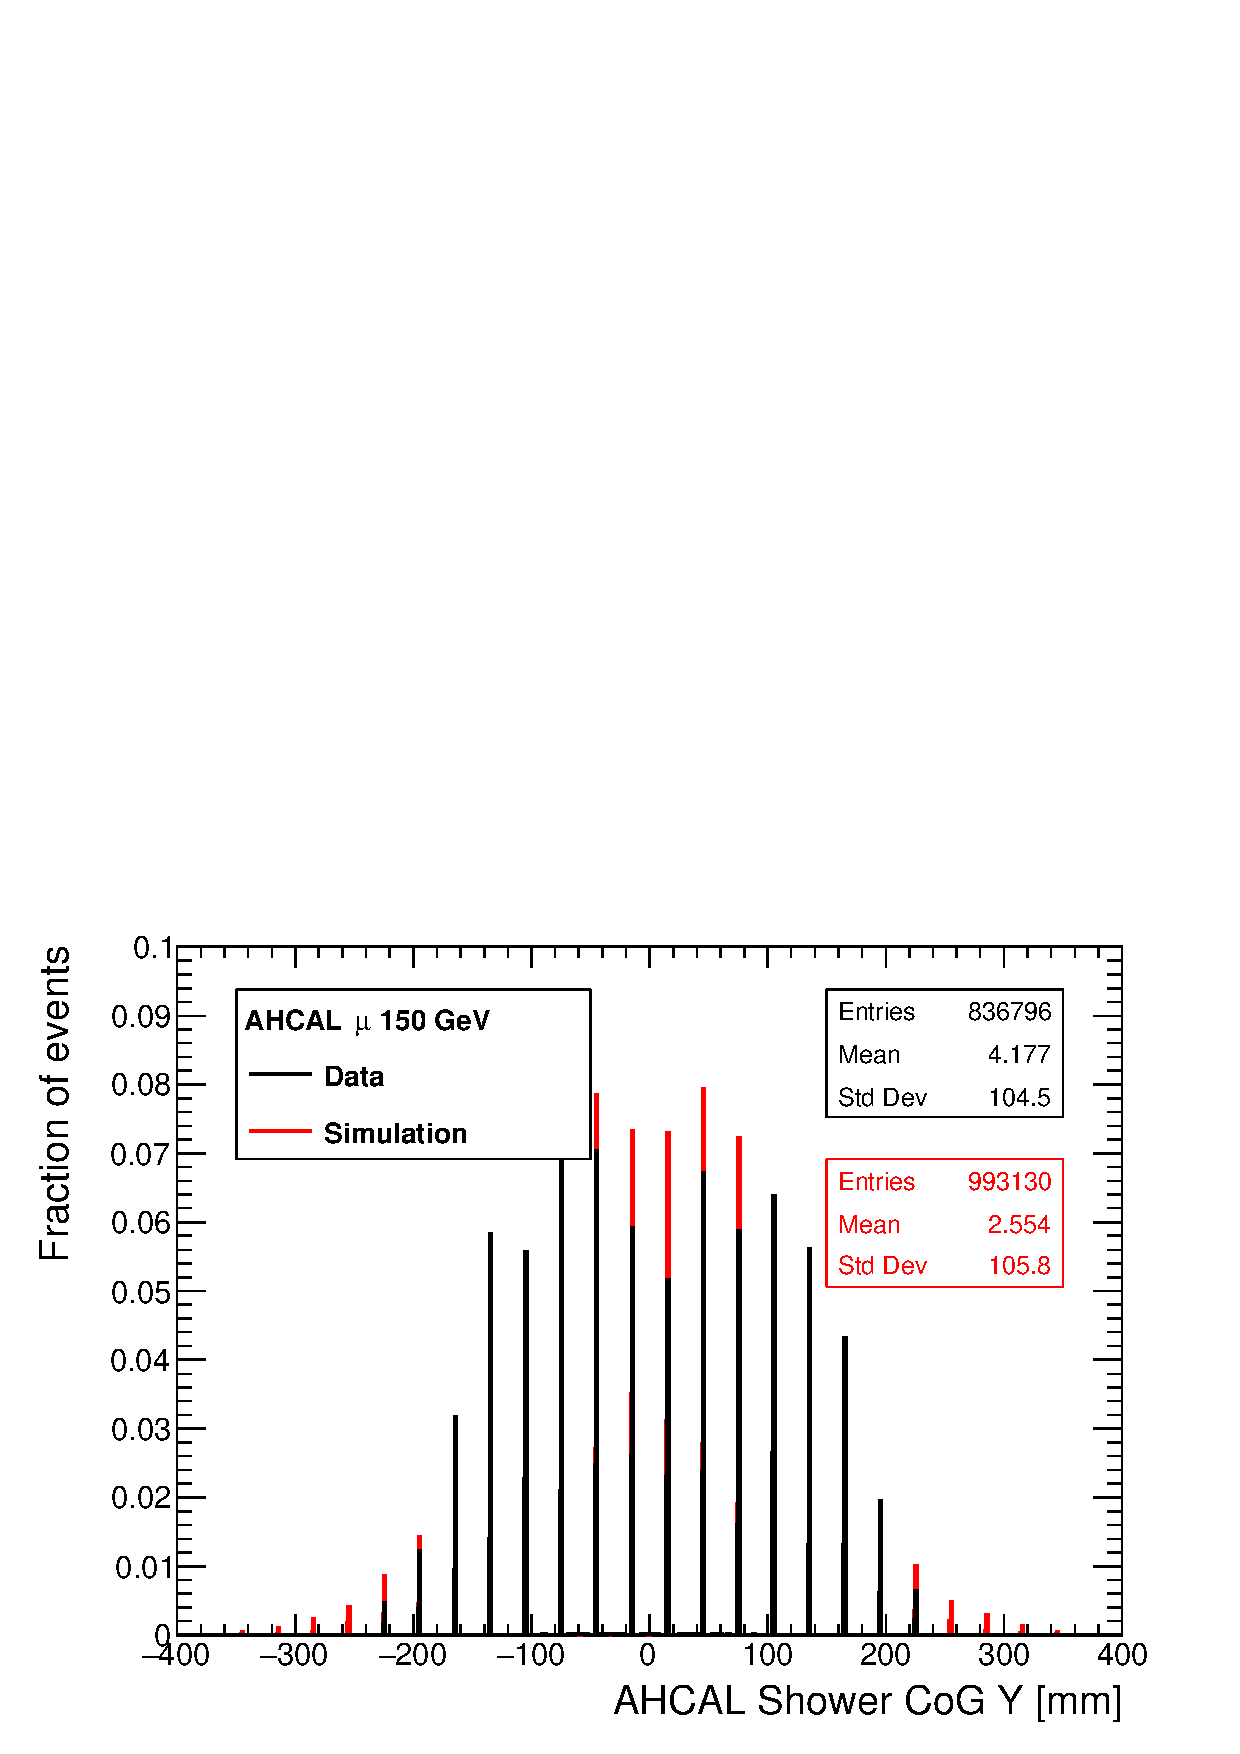
\includegraphics[width=1.\linewidth]{../Thesis_Plots/Timing/Muons/Plots/BeamProfileY.pdf}
    \caption{Beam profile X=Y.} \label{fig:mu150GeVY}
  \end{subfigure}
  \caption{Beam profiles for 150 GeV muons in data and simulation. Simulated with QGSP\_BERT\_HP using \geant v10.1.}
  \label{fig:BPmu}
\end{figure}

\begin{figure}[htbp!]
  \centering
  \begin{subfigure}[t]{0.49\textwidth}
    \includegraphics[width=1.\linewidth]{../Thesis_Plots/Timing/Electrons/Plots/Run24405_CoGX_AHCAL_50GeV_Comparison.pdf}
    \caption{Beam profile X.} \label{fig:e50GeVX}
  \end{subfigure}
  \hfill
  \begin{subfigure}[t]{0.49\textwidth}
    \includegraphics[width=1.\linewidth]{../Thesis_Plots/Timing/Electrons/Plots/Run24405_CoGY_AHCAL_50GeV_Comparison.pdf}
    \caption{Beam profile Y.} \label{fig:e50GeVY}
  \end{subfigure}
  \caption{Beam profiles for 50 GeV electrons in data and simulation. Simulated with QGSP\_BERT\_HP using \geant v10.1.}
\end{figure}

\begin{figure}[htbp!]
  \centering
  \begin{subfigure}[t]{0.49\textwidth}
    \includegraphics[width=1.\linewidth]{../Thesis_Plots/Timing/Pions/Plots/Run24332_CoGX_AHCAL_90GeV_Comparison.pdf}
    \caption{90 GeV.} \label{fig:pi90GeVX}
  \end{subfigure}
  \hfill
  \begin{subfigure}[t]{0.49\textwidth}
    \includegraphics[width=1.\linewidth]{../Thesis_Plots/Timing/Pions/Plots/Run24332_CoGY_AHCAL_90GeV_Comparison.pdf}
    \caption{90 GeV.} \label{fig:pi90GeVY}
  \end{subfigure}
  \caption{Beam profiles for 90 GeV pions in data and simulation. Simulated with QGSP\_BERT\_HP using \geant v10.1.}
\end{figure}

\begin{figure}[htbp!]
  \centering
  \begin{subfigure}[t]{0.49\textwidth}
    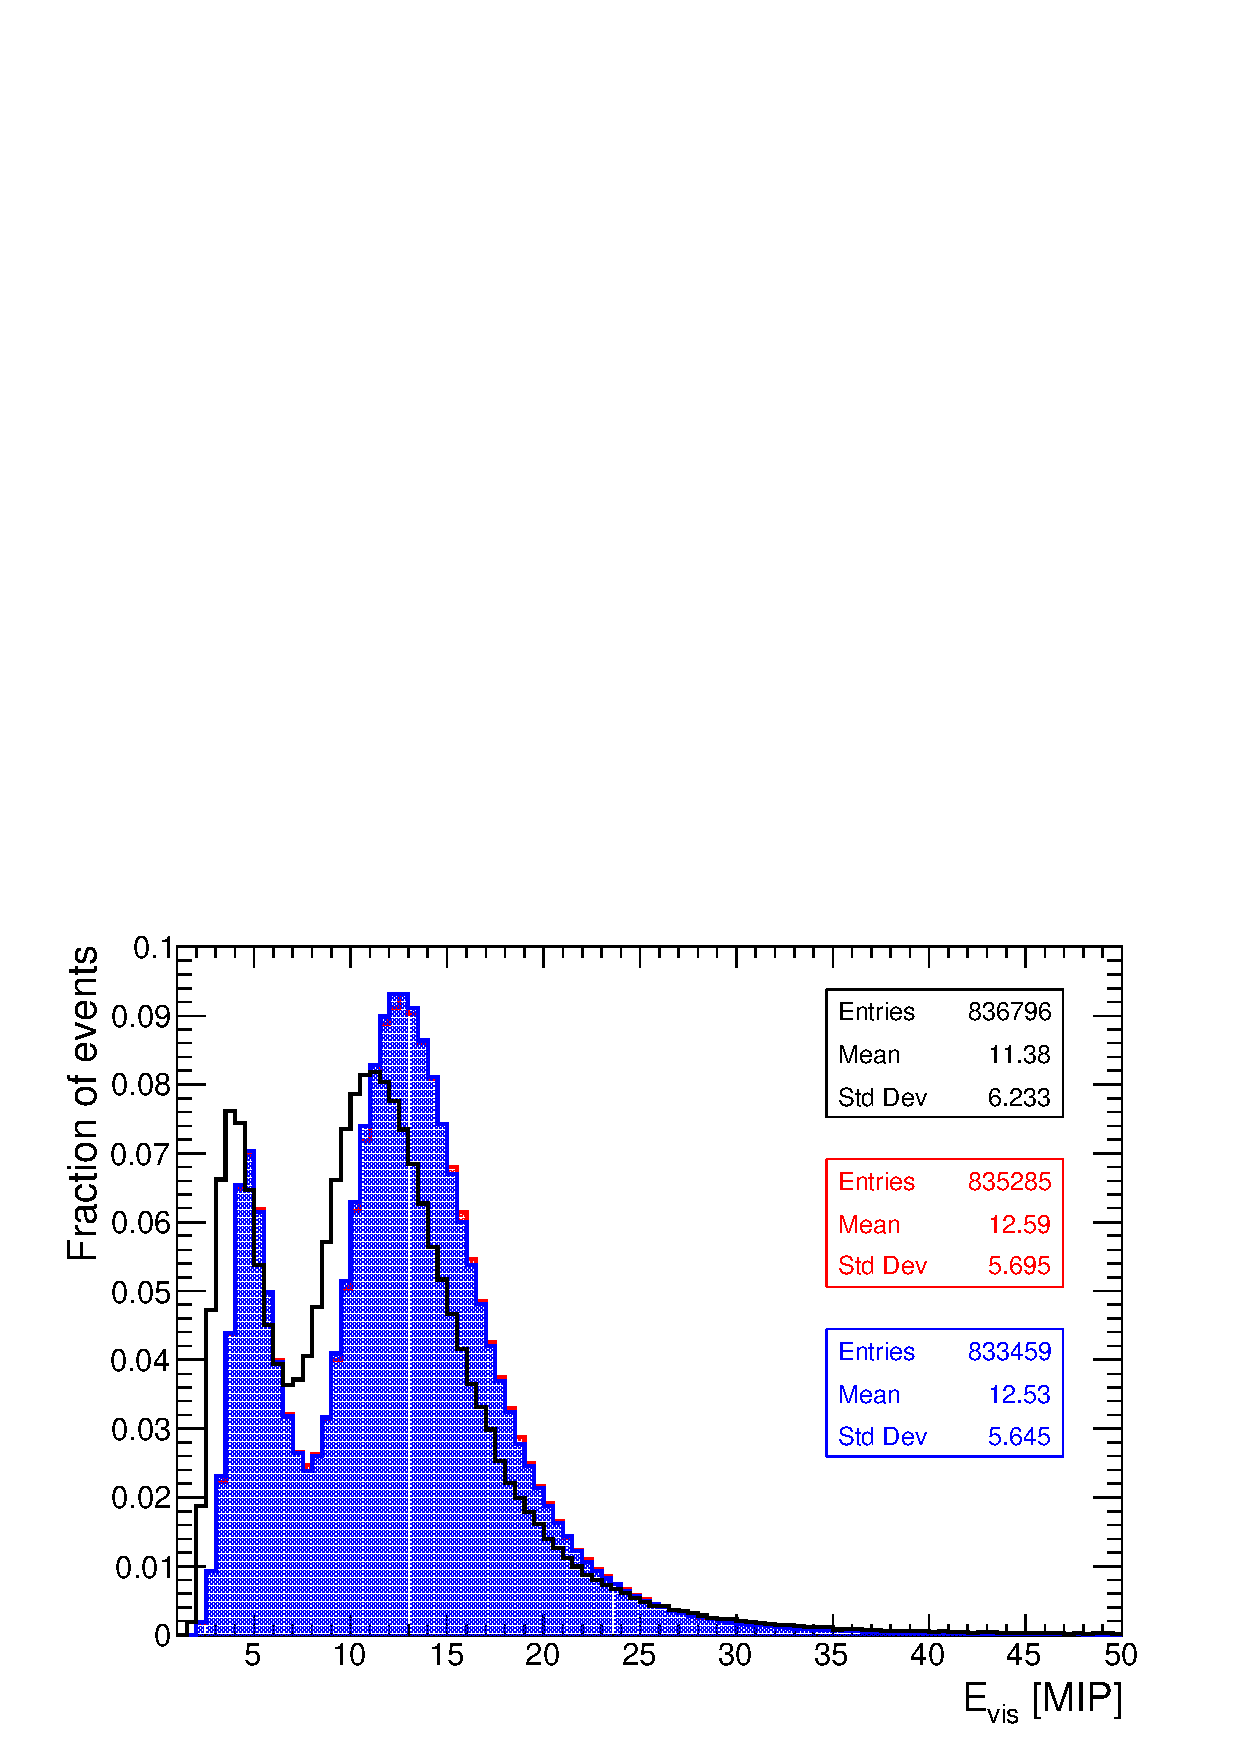
\includegraphics[width=1.\linewidth]{../Thesis_Plots/Timing/Muons/Plots/Validation_Evis_Muons.pdf}
    \caption{$E_{sum}$.} \label{fig:muEvis}
  \end{subfigure}
  \hfill
  \begin{subfigure}[t]{0.49\textwidth}
    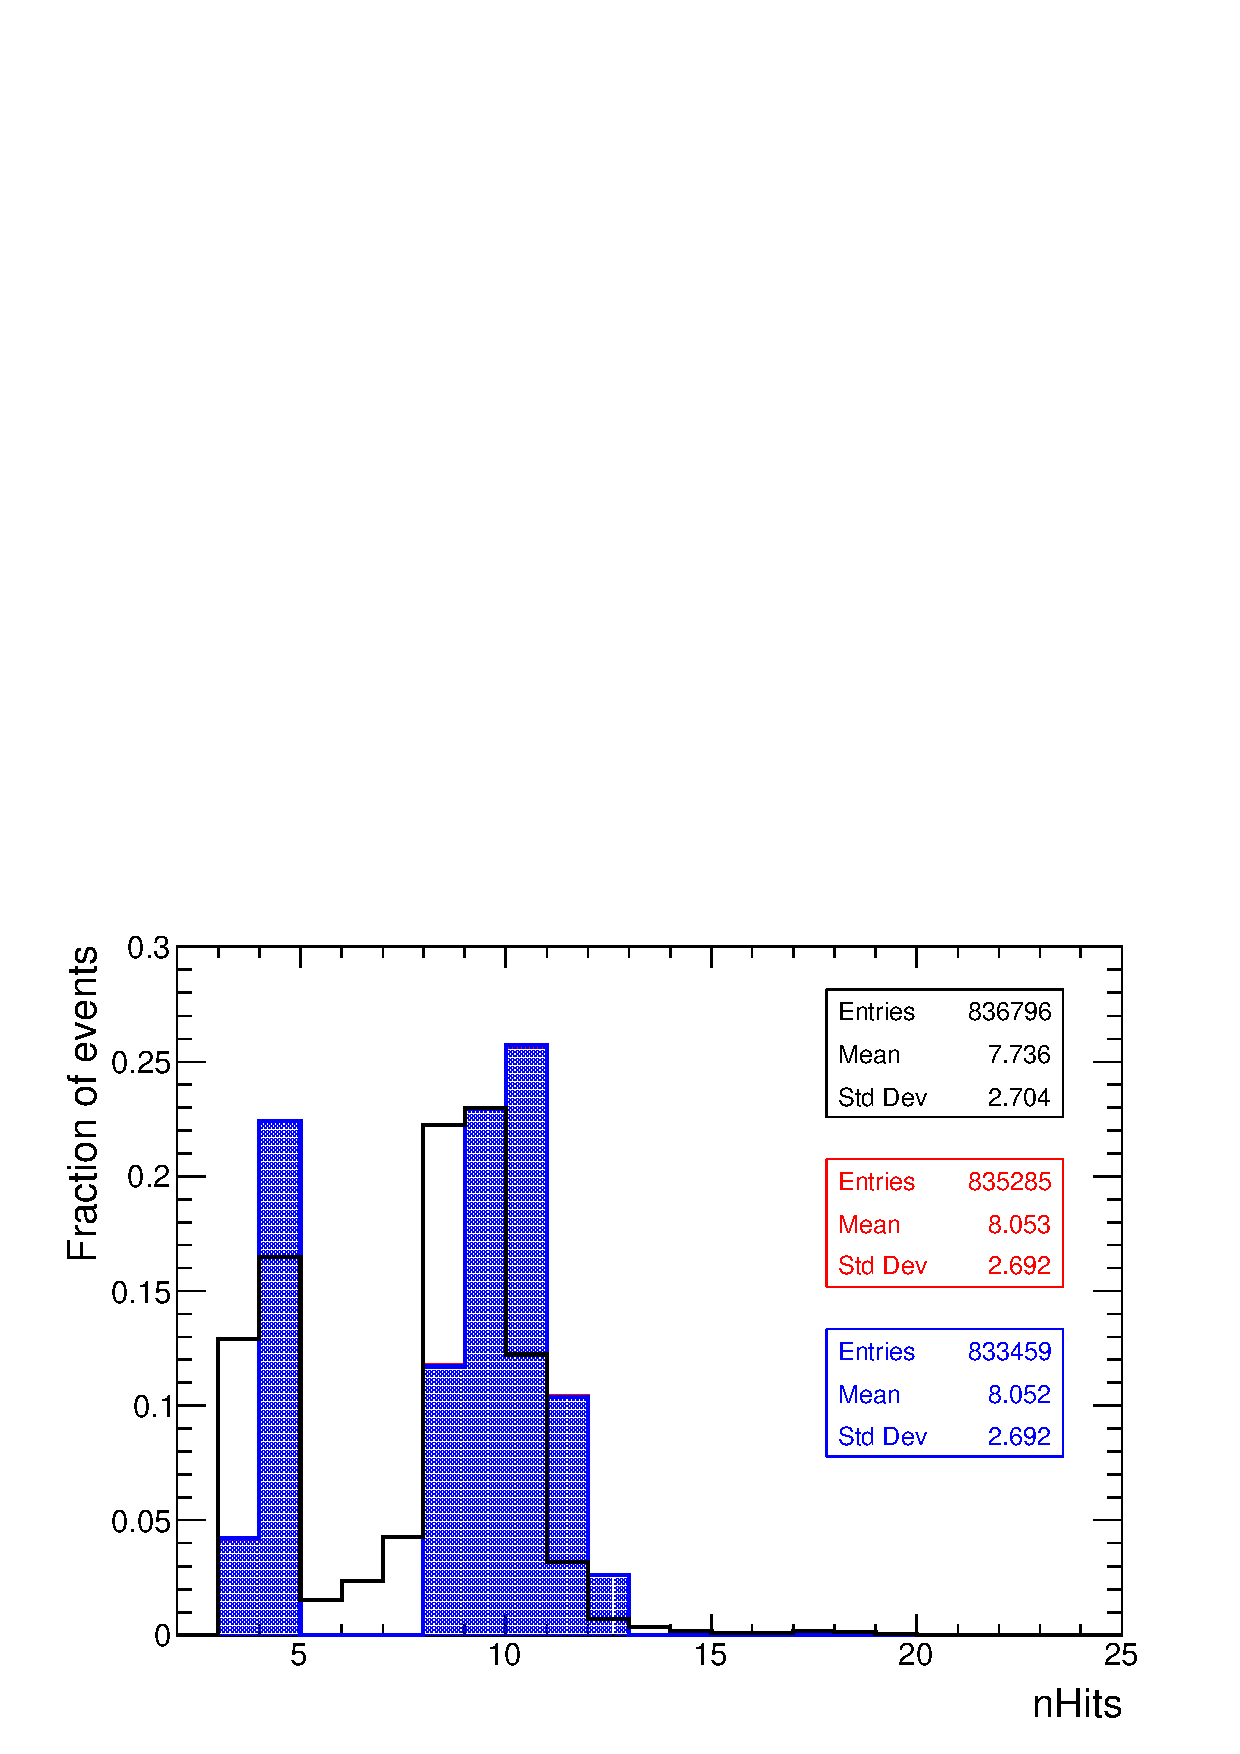
\includegraphics[width=1.\linewidth]{../Thesis_Plots/Timing/Muons/Plots/Validation_nHits_Muons.pdf}
    \caption{nHits.} \label{fig:munHits}
  \end{subfigure}
  \caption{\subref{fig:muEvis}) The energy sum in the AHCAL for 150 GeV muons in data and simulations. \subref{fig:munHits}) The number of hits in the AHCAL for 150 GeV muons in data and simulations.}
  \label{fig:muVal}
\end{figure}

\begin{figure}[htbp!]
	\centering
	\begin{subfigure}[t]{0.49\textwidth}
		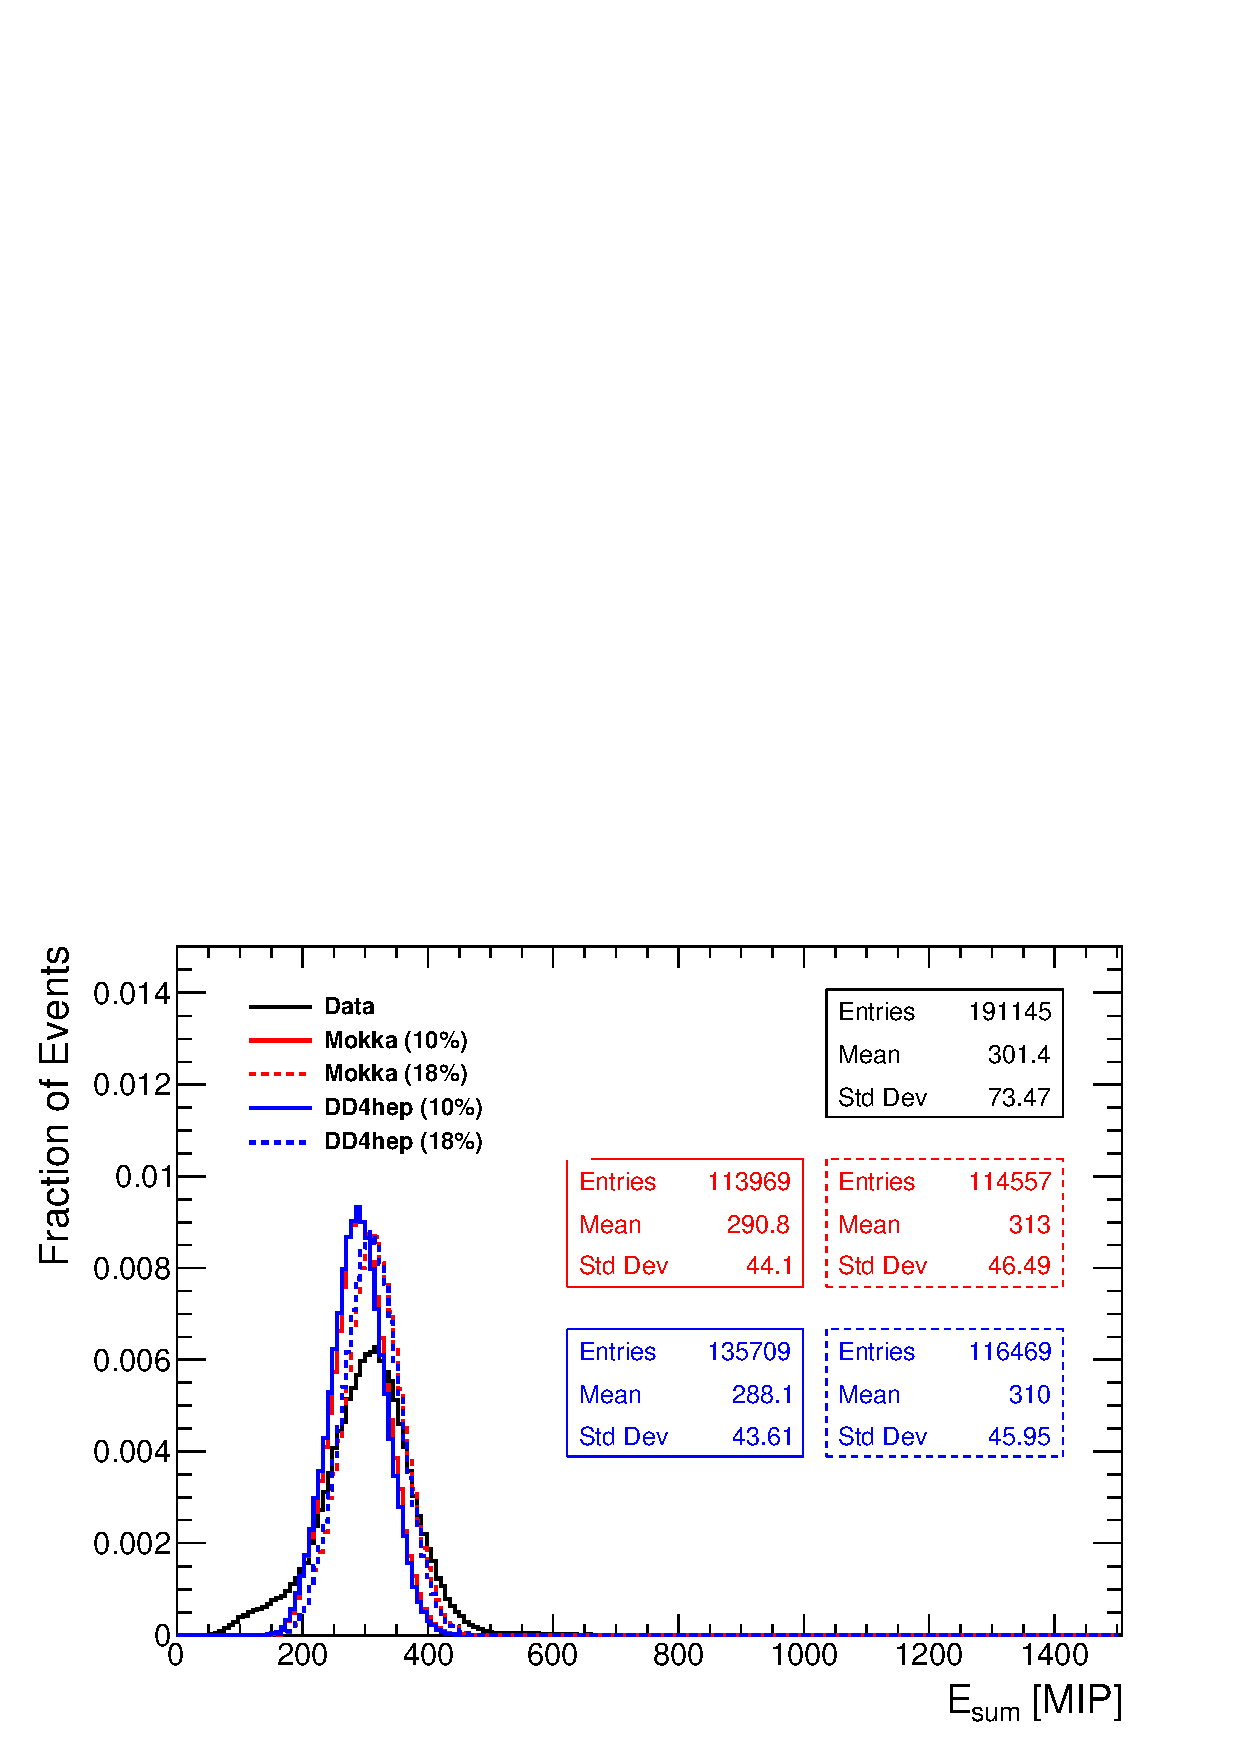
\includegraphics[width=1.\linewidth]{../Thesis_Plots/Timing/Electrons/Plots/Comparison_EnergySum_Xtalk_electrons10GeV.pdf}
		\caption{$E_{sum}$.} \label{fig:e10Evis}
	\end{subfigure}
	\hfill
	\begin{subfigure}[t]{0.49\textwidth}
		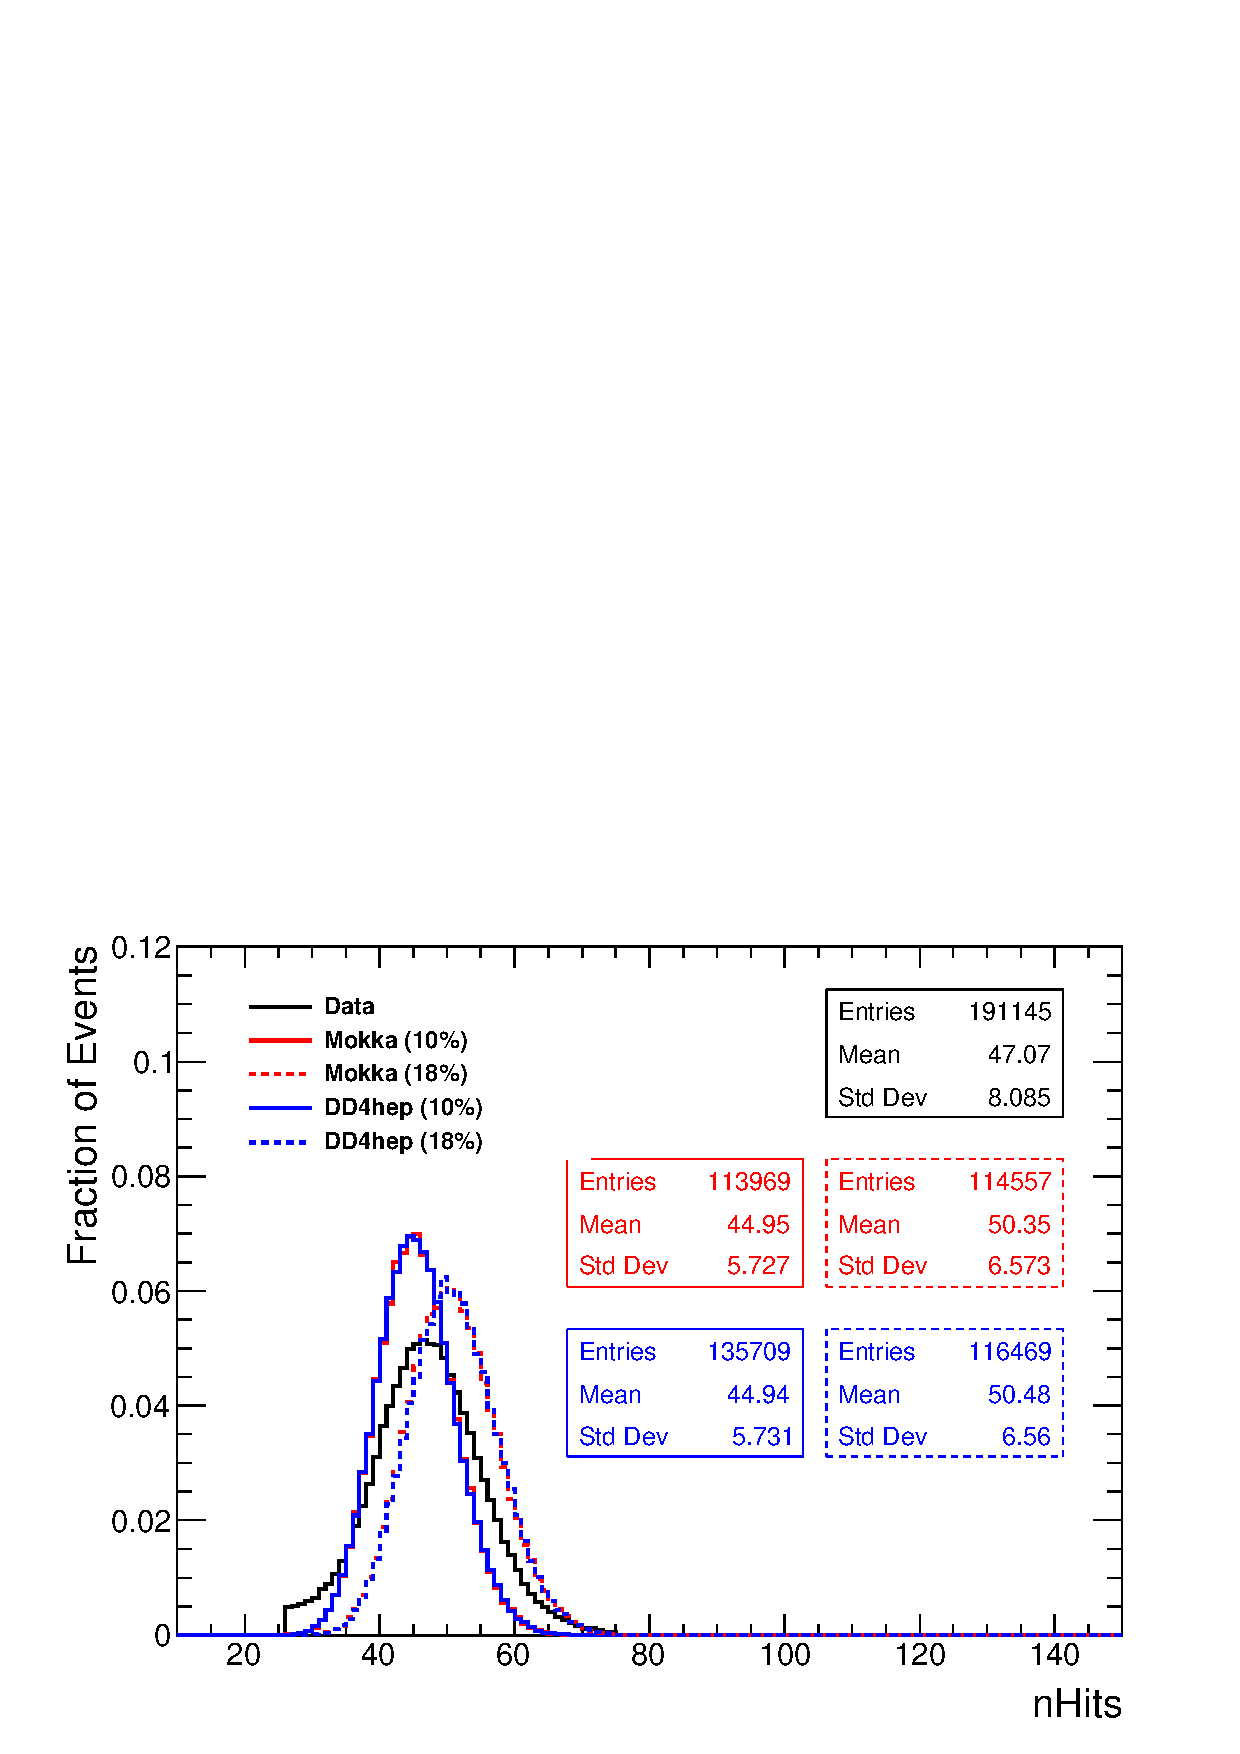
\includegraphics[width=1.\linewidth]{../Thesis_Plots/Timing/Electrons/Plots/Comparison_nHits_Xtalk_electrons10GeV.pdf}
		\caption{nHits.} \label{fig:e10nHits}
	\end{subfigure}
	\caption{\subref{fig:e10Evis}) The energy sum in the AHCAL for 10 GeV electrons for data and simulations with a cross-talk value of 10\% and 18\%. \subref{fig:e10nHits}) The number of hits in the AHCAL for 10 GeV electrons for data and simulations with a cross-talk value of 10\% and 18\%.}
	\label{fig:e10Val}
\end{figure}

\begin{figure}[htbp!]
	\centering
	\begin{subfigure}[t]{0.49\textwidth}
		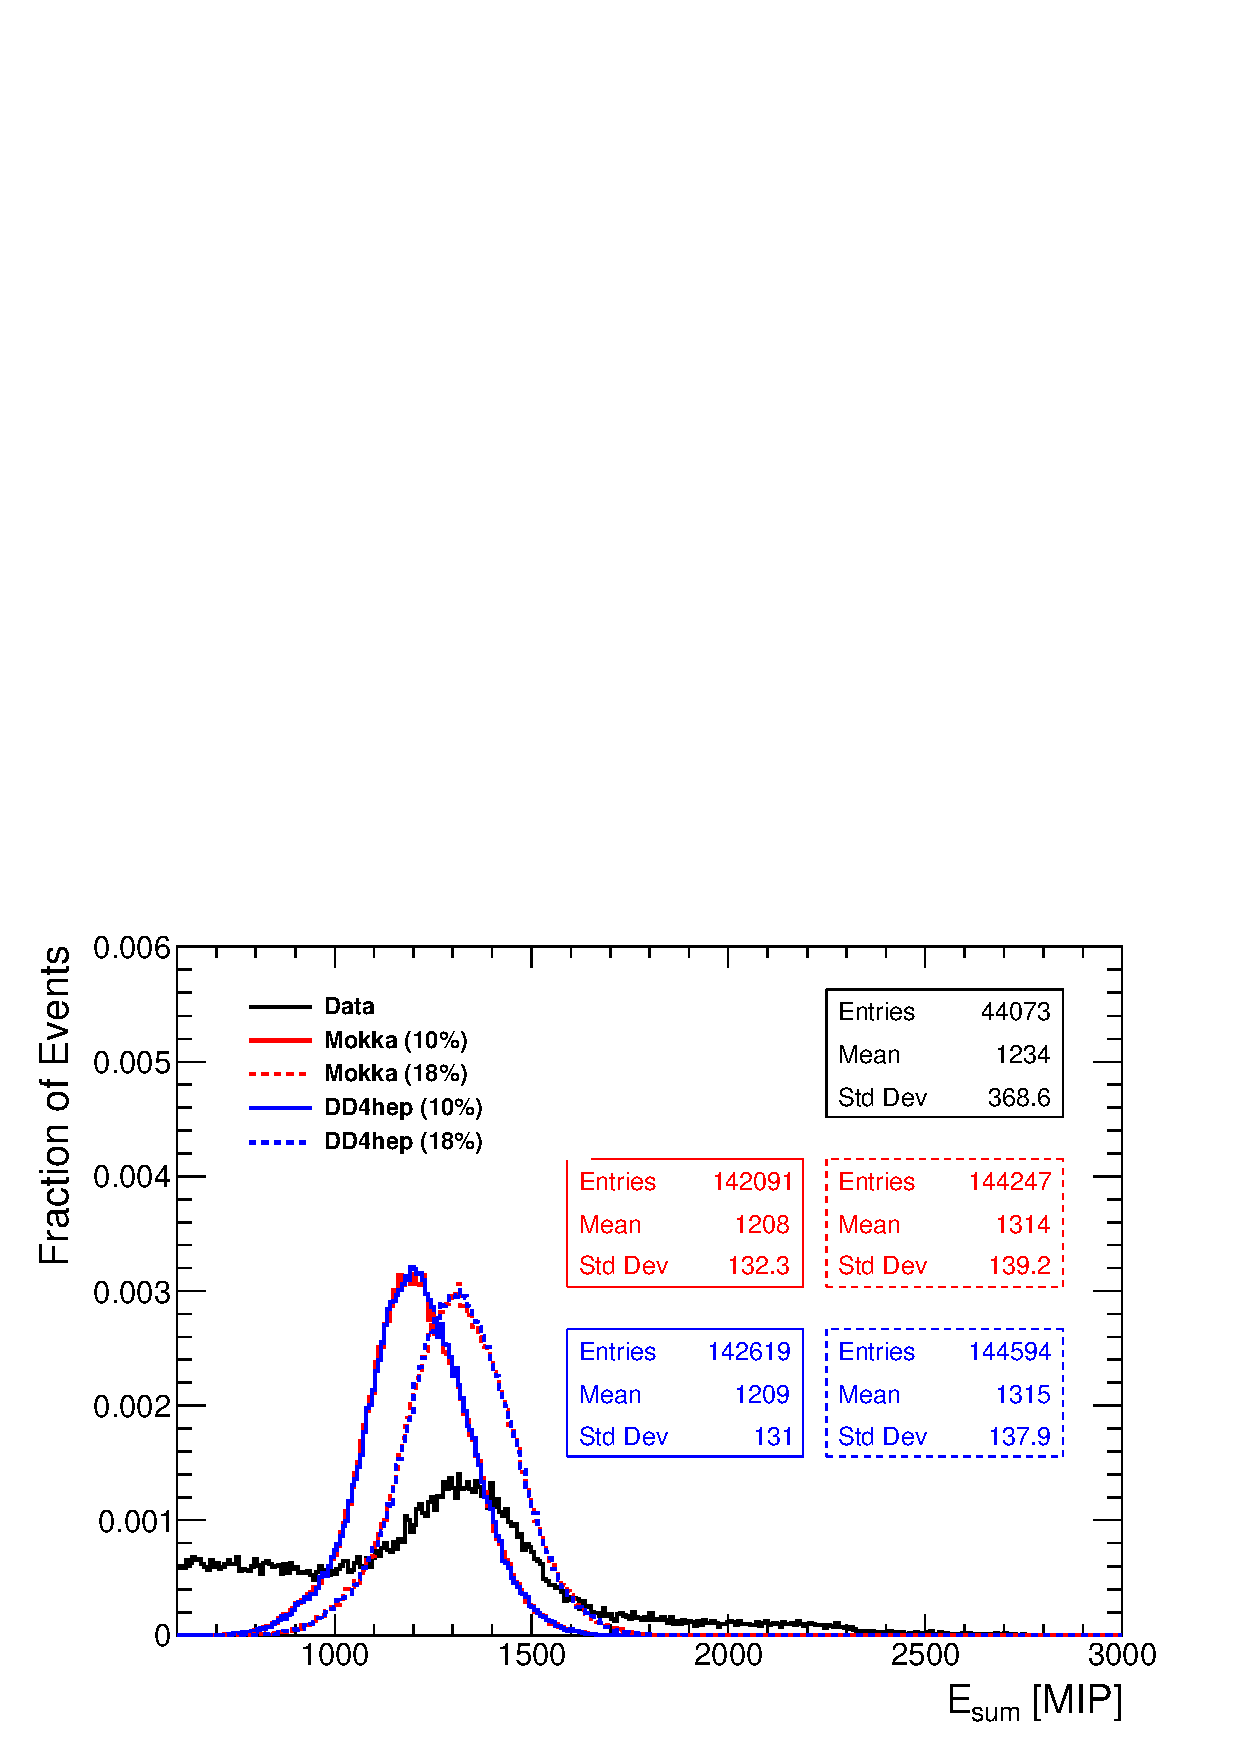
\includegraphics[width=1.\linewidth]{../Thesis_Plots/Timing/Electrons/Plots/Comparison_EnergySum_Xtalk_electrons50GeV.pdf}
		\caption{$E_{sum}$.} \label{fig:e50Evis}
	\end{subfigure}
	\hfill
	\begin{subfigure}[t]{0.49\textwidth}
		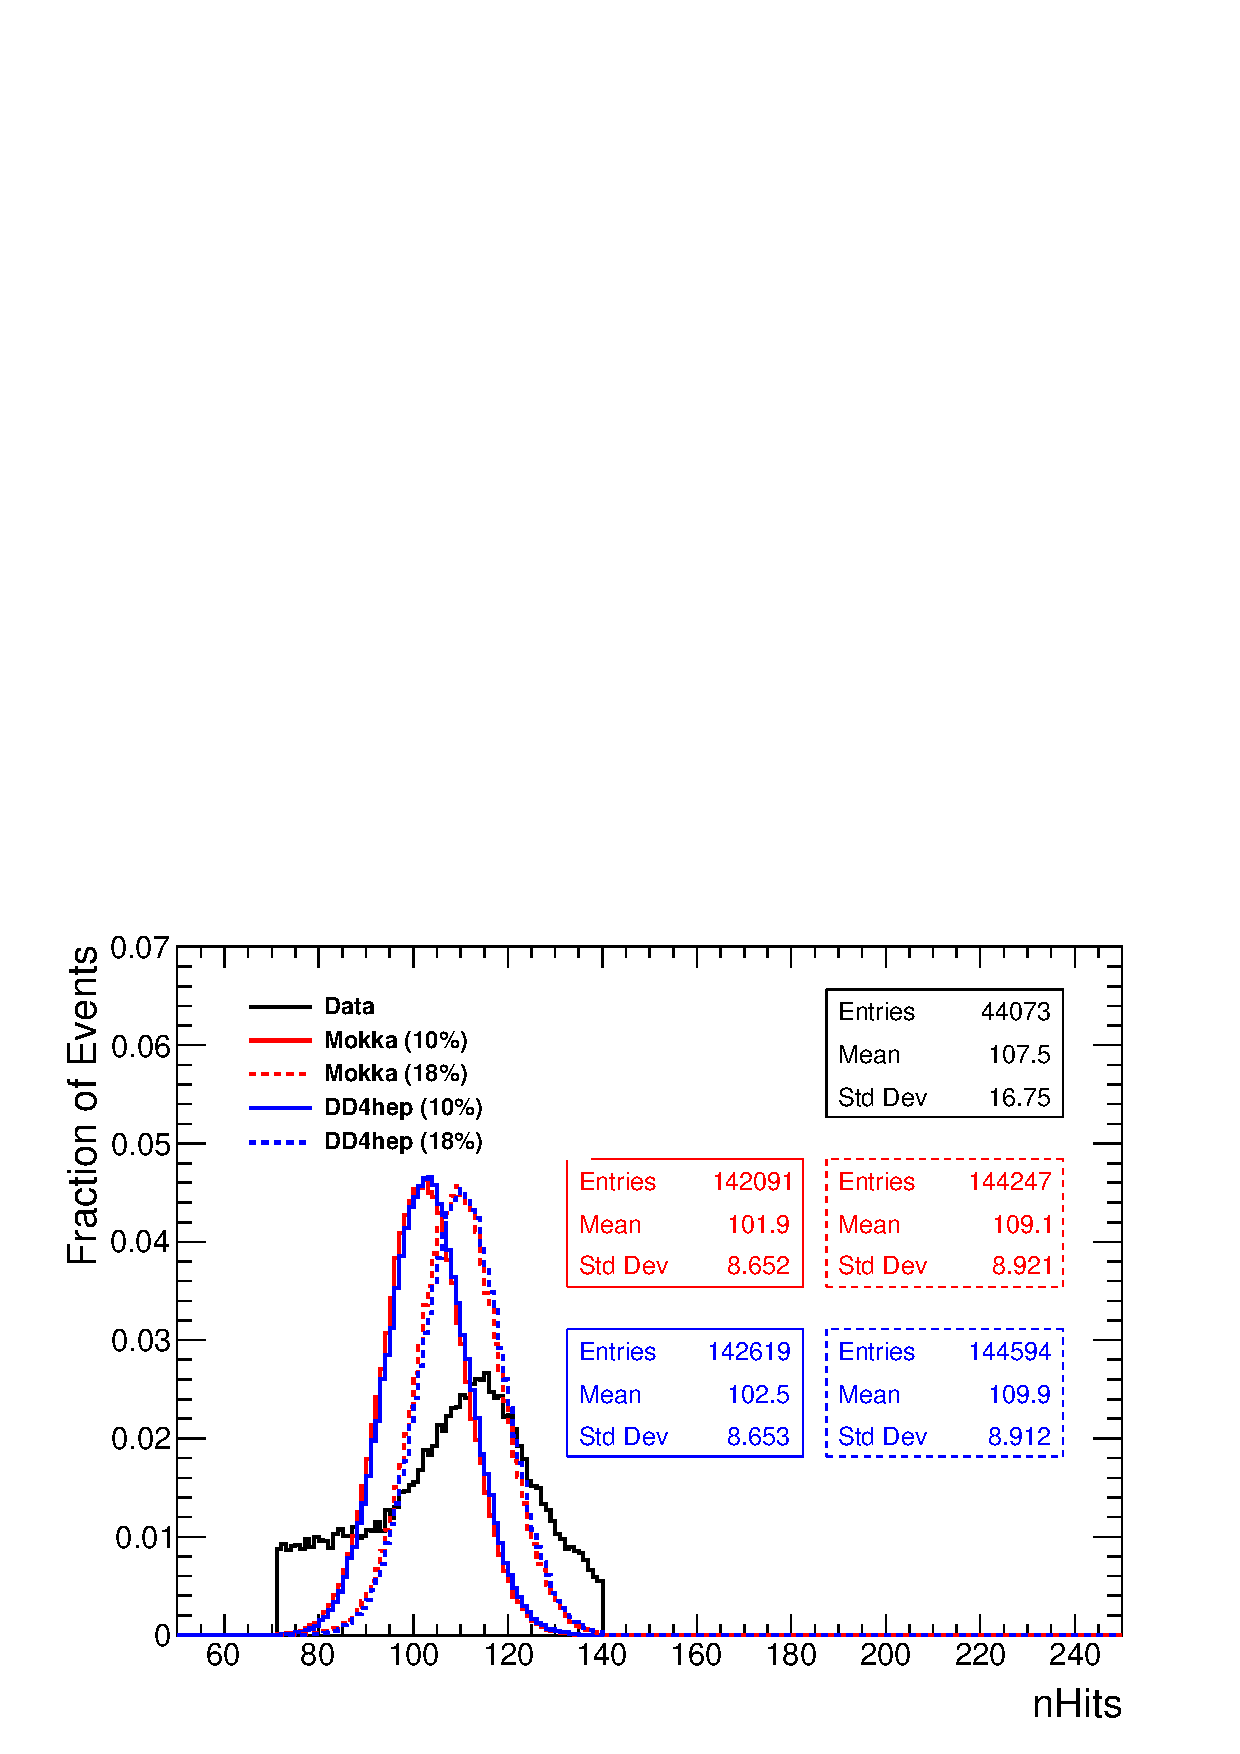
\includegraphics[width=1.\linewidth]{../Thesis_Plots/Timing/Electrons/Plots/Comparison_nHits_Xtalk_electrons50GeV.pdf}
		\caption{nHits.} \label{fig:e50nHits}
	\end{subfigure}
	\caption{\subref{fig:e50Evis}) The energy sum in the AHCAL for 50 GeV electrons for data and simulations with a cross-talk value of 10\% and 18\%. \subref{fig:e50nHits}) The number of hits in the AHCAL for 50 GeV electrons for data and simulations with a cross-talk value of 10\% and 18\%.}
	\label{fig:e50Val}
\end{figure}
